%----------------------------------------------------------------------------
% Magic tutorial number 7
%----------------------------------------------------------------------------

\NeedsTeXFormat{LaTeX2e}[1994/12/01]
\documentclass[letterpaper,twoside,12pt]{article}
\usepackage{epsfig,times}

\setlength{\textwidth}{8.5in}
\addtolength{\textwidth}{-2.0in}
\setlength{\textheight}{11.0in}
\addtolength{\textheight}{-2.0in}
\setlength{\oddsidemargin}{0in}
\setlength{\evensidemargin}{0pt}
\setlength{\topmargin}{-0.5in}
\setlength{\headheight}{0.2in}
\setlength{\headsep}{0.3in}
\setlength{\topskip}{0pt}

\def\hinch{\hspace*{0.5in}}
\def\starti{\begin{center}\begin{tabbing}\hinch\=\hinch\=\hinch\=hinch\hinch\=\kill}
\def\endi{\end{tabbing}\end{center}}
\def\ii{\>\>\>}
\def\mytitle{Magic Tutorial \#7: Netlists and Routing}

%----------------------------------------------------------------------------

\begin{document}

\makeatletter
\newcommand{\ps@magic}{%
	\renewcommand{\@oddhead}{\mytitle\hfil\today}%
	\renewcommand{\@evenhead}{\today\hfil\mytitle}%
	\renewcommand{\@evenfoot}{\hfil\textrm{--{\thepage}--}\hfil}%
	\renewcommand{\@oddfoot}{\@evenfoot}}
\newcommand{\ps@mplain}{%
	\renewcommand{\@oddhead}{}%
	\renewcommand{\@evenhead}{}%
	\renewcommand{\@evenfoot}{\hfil\textrm{--{\thepage}--}\hfil}%
	\renewcommand{\@oddfoot}{\@evenfoot}}
\makeatother
\pagestyle{magic}
\thispagestyle{mplain}


\begin{center}
  {\bfseries \Large \mytitle} \\
  \vspace*{0.5in}
  {\itshape John Ousterhout} \\
  \vspace*{0.5in}
   Computer Science Division \\
   Electrical Engineering and Computer Sciences \\
   University of California \\
   Berkeley, CA  94720 \\
  \vspace*{0.25in}
  {\itshape (Updated by others, too.)} \\
  \vspace*{0.25in}
  This tutorial corresponds to Magic version 7. \\
\end{center}
\vspace*{0.5in}

{\noindent\bfseries\large Tutorials to read first:}
\starti
   \> Magic Tutorial  \#1: Getting Started \\
   \> Magic Tutorial \#2: Basic Painting and Selection \\
   \> Magic Tutorial \#3: Advanced Painting (Wiring and Plowing) \\
   \> Magic Tutorial \#4: Cell Hierarchies \\
   \> Magic Tutorial \#5: Multiple Windows \\
\endi

{\noindent\bfseries\large Netlist Commands introduced in this tutorial:}
\starti
   \> :extract, :flush, :ripup, :savenetlist, :trace, :writeall
\endi

{\noindent\bfseries\large Layout Commands introduced in this tutorial:}
\starti
   \> :channel, :route
\endi

{\noindent\bfseries\large Macros introduced in this tutorial:}

\starti
   \> {\itshape (none)}
\endi

\vspace*{0.75in}
\section{Introduction}

This tutorial describes how to use Magic's automatic routing
tools to make interconnections between subcells in a design.  In
addition to the standard Magic router, which is invoked by the {\bfseries route}
command and covered in this tutorial, two
other routing tools are available.  A gate-array router {\itshape Garouter}
permits user specified channel definitions, terminals in the interior
of cells, and route-throughs across cells.  To learn about the gate-array
router read this first then
``Magic Tutorial \#12:  Routing Gate Arrays''.  Finally Magic
provides an interactive maze-router that takes graphic hints, the 
{\itshape Irouter}, that
permits the user to control the overall path of routes while leaving
the tedious details to Magic.  The {\itshape Irouter} is documented in 
``Magic Tutorial \#10:  The Interactive Router''.

The standard Magic router provides an {\itshape obstacle-avoidance}
capability:  if there is mask material in
the routing areas, the router can work under, over, or
around that material to complete the connections.  This means
that you can pre-route key signals by hand and have Magic
route the less important signals automatically.  In addition,
you can route power and ground by hand (right now we don't have
any power-ground routing tools, so you {\itshape have}
to route them by hand).

The router {\itshape only} makes connections between
subcells; to make point-to-point connections between pieces of layout within
a single cell you should use the wiring command described
in ``Magic Tutorial \#3: Advanced Painting (Wiring and Plowing) '' or
the maze router described in ``Magic Tutorial \#10:  The Interactive Router''.
If you only need to make a few connections you are probably better off doing
them manually.

The first step in routing is to tell Magic what should be connected
to what.  This information is contained in a file called a {\itshape netlist}.
Sections 2, 3, 4, and 5 describe how to create and modify netlists using
Magic's interactive netlist editing tools.
Once you've created a netlist, the next step is to invoke the
router.  Section 6 shows how to do this, and gives a brief summary
of what goes on inside the routing tools.  Unless your design is
very simple and has lots of free space, the routing probably won't
succeed the first time.  Section 7 describes the feedback provided
by the routing tools.  Sections 8 and 9 discuss how you can modify your design
in light of this feedback to improve its routability.
You'll probably need to iterate a few times until the routing is successful.

\section{Terminals and Netlists}

A netlist is a file that describes a set of desired connections.
It contains one or more {\itshape nets}.  Each net names a
set of {\itshape terminals} that should all be wired together.
A terminal is simply a label attached to a piece of mask material within
a subcell; it is distinguishable from ordinary labels within a subcell by its
presence within a netlist file and by certain characteristics
common to terminals, as described below.

The first step in building a netlist is to label the terminals in
your design.  Figure 1 shows an example.  Each label should
be a line or rectangle running along the edge of the cell (point terminals
are not allowed).
The router will make a connection to the cell somewhere along a
terminal's length.
If the label isn't at the edge of the cell,
Magic will route recklessly across the cell to reach the terminal,
taking the shortest path between the terminal and a routing channel.
It's almost always a good idea to arrange for terminal labels to
be at cell edges.  The label must be at least as wide as the minimum width
of the routing material;  the wider you make the label, the more flexibility
you give the router to choose a good point to connect to the terminal.

\begin{figure}[ht]
   \begin{center}
      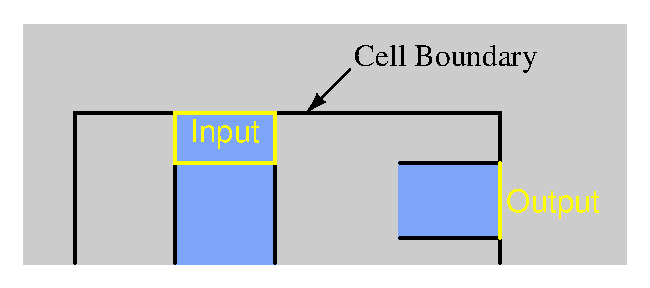
\epsfig{file=../psfigures/tut7.1.ps, width=0.5\columnwidth}
      \caption{An example of terminal labels.  Each terminal
	should be labeled with a line or rectangle along the
	edge of the cell.}
   \end{center}
\end{figure}

Terminal labels must be attached to mask material that connects
directly to one of Magic's two routing layers (Routing layers are defined
in Magic's technology file).
For example, in the SCMOS process
where the routing layers are metal1 and metal2, diffusion
may not be used as a terminal since neither of the routing
layers will connect directly to it.  On the other hand, a terminal
may be attached to diffusion-metal1 contact, since the metal1 routing layer
will connect properly to it.
Terminals can have arbitrary names, except that they should not
contain slashes (``/'') or the substring ``feedthrough'', and should not
end in ``@'', ``\$'', or ``\^{}''.
See Tutorial \#2 for a complete description of labeling conventions.

For an example of good and bad terminals, edit the cell {\bfseries tut7a}.
The cell doesn't
make any electrical sense, but contains several good and bad
terminals.
All the terminals with names like {\bfseries bad1} are incorrect or
undesirable for one of the reasons given above, and those with
names like {\bfseries good4} are acceptable.

\begin{figure}[ht]
   \begin{center}
      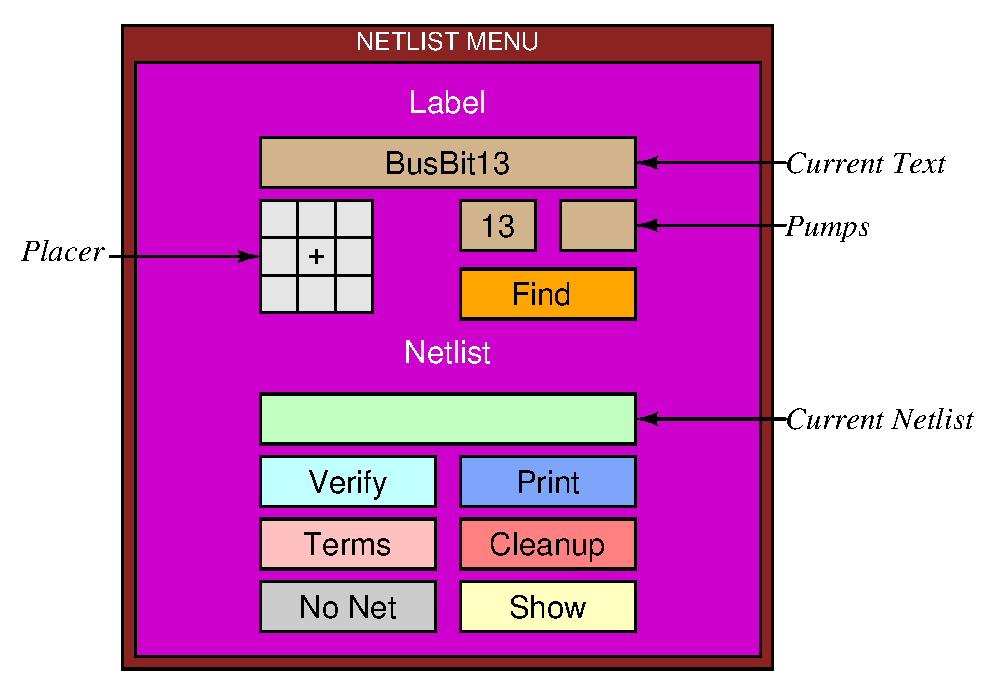
\epsfig{file=../psfigures/tut7.2.ps, width=0.7\columnwidth}
      \caption{The netlist menu.}
   \end{center}
\end{figure}

\begin{table}[ht]
   \begin{center}
      \begin{tabular}{|l|l|} \hline
	Button	& Action \\ \hline
	Current Text	& Left-click:  prompt for more labels \\
			& Right-click:  advance to next label \\ \hline
	Placer		& Left-click:  place label \\
			& Right-click:  change label text position \\ \hline
	Pumps		& Left-click:  decrement number \\
			& Right-click:  increment number \\ \hline
	Find		& Search under box, highlight labels \\
			& matching current text \\ \hline
	Current Netlist	& Left-click:  prompt for new netlist name \\
			& Right-click:  use edit cell name as netlist name \\ \hline
	Verify		& Check that wiring matches netlist (same as \\
			& typing {\bfseries :verify} command) \\ \hline
	Print		& Print names of all terminals in selected net \\
			& (same as typing {\bfseries :print} command) \\ \hline
	Terms		& Place feedback areas on screen to identify all terminals \\
			& in current netlist (same as {\bfseries :showterms} command) \\
				\hline
	Cleanup		& Check current netlist for missing labels and nets \\
			& with less than two terminals (same as typing \\ \hline
			& {\bfseries :cleanup} command) \\
	No Net		& Delete selected net (same as {\bfseries :dnet} command) \\
				\hline
	Show		& Highlight paint connected to material under box \\
			& (same as typing {\bfseries :shownet} command) \\ \hline
      \end{tabular}
      \caption{A summary of all the netlist menu button actions.}
   \end{center}
\end{table}

If you create two or more terminal labels with the same name in the same cell
the router will assume that they are electrically equivalent (connected
together within the cell).
Because of this, when routing the net it will feel free to connect to
whichever one of the terminals is most convenient, and ignore the others.
In some cases the router may take advantage of electrically equivalent
terminals by using {\itshape feed throughs}: entering a cell at one terminal to make
one connection, and exiting through an equivalent terminal on the way to make
another connection for the same net.

\section{Menu for Label Editing}

Magic provides a special menu facility to assist you in placing terminal labels
and editing netlists.  To make the menu appear, invoke the Magic command

\starti
   \ii {\bfseries :specialopen netlist}
\endi

A new window will appear in the lower-left corner of the screen,
containing several rectangular areas on a purple background.  Each
of the rectangular areas is called a {\itshape button}.  Clicking
mouse buttons inside the menu buttons will invoke various
commands to edit labels and netlists.
Figure 2 shows a diagram of the netlist menu and Table I summarizes
the meaning of button clicks in various menu items.
The netlist menu can be grown, shrunk, and moved just like any other
window;  see ``Magic Tutorial \#5: Multiple Windows'' for details.
It also has its own private set of commands.  To see what commands
you can type in the netlist menu, move the cursor over the menu and
type

\starti
   \ii {\bfseries :help}
\endi

You shouldn't need to type commands in the netlist menu very often,
since almost everything you'll need to do can be done using
the menu.  See Section 9 for a description of a few of the commands you
can type;  the complete set is described in the manual
page {\itshape magic(1)}.  One of the best uses for the commands is so
that you can define macros for them and avoid having to go back and
forth to the menu;  look up the {\bfseries :send} command in the man page
to see how to do this.
The top half of the
menu is for placing labels and the bottom half is for editing
netlists.  This section describes the
label facilities, and Section 4 describes the netlist facilities.

The label menu makes it easy for you to enter lots
of labels, particularly when there are many labels that are the
same except for a number, e.g. {\bfseries bus1}, {\bfseries bus2}, {\bfseries bus3},
etc.  There are four sections to the label menu:  the current text,
the placer, two pumps, and the {\bfseries Find} button.  To place labels,
first click the left mouse button over the current text rectangle.
Then type one or more labels on the keyboard, one per
line.  You can use this mechanism to enter several labels at once.
Type return twice to signal the end of
the list.  At this point, the first of the labels you typed will
appear in the current text rectangle.

To place a label, position the box over the area you want to label,
then click the left mouse button inside one of the squares of the
placer area.  A label will be created with the current text.
Where you click in the placer determines where the label text
will appear relative to the label box:  for example, clicking the left-center
square causes the text to be centered just to the left of the box.
You can place many copies of the same label by moving the box and
clicking the placer area again.  You can
re-orient the text of a label by clicking the right mouse button
inside the placer area.  For example, if you would like to
move a label's text so that it appears centered above the label,
place the box over the label and right-click the top-center placer
square.

If you entered several labels at once, only the first appears in
the current text area.  However, you can advance to the next label
by right-clicking inside the current text area.  In this way you
can place a long series of labels entirely with the mouse.  Try
using this mechanism to add labels to {\bfseries tut7a}.

The two small buttons underneath the right side of the current
text area are called pumps.  To see how these work, enter a label
name containing a number into the current text area, for example,
{\bfseries bus1}.  When you do this, the ``1'' appears in the left
pump.  Right-clicking the pump causes the number to increment,
and left-clicking the pump causes the number to decrement.  This
makes it easy for you to enter a series of numbered signal names.
If a name has two numbers in it, the second number will appear in
the second pump, and it can be incremented or decremented too.
Try using the pumps to place a series of numbered names.

The last entry in the label portion of the menu is the {\bfseries Find}
button.  This can be used to locate a label by searching for
a given pattern.  If you click the {\bfseries Find} button, Magic
will use the current text as a pattern and
search the area underneath the box for a label whose name
contains the pattern.  Pattern-matching is done in the same
way as in {\itshape csh}, using the special characters ``*'',
``?'', ``\\'', ``['', and ``]''.  Try this on {\bfseries tut7a}:
enter ``good*'' into the current text area, place the box around
the whole cell, then click on the ``Find'' button.  For each of
the good labels, a feedback area will be created with white
stripes to highlight the area.  The {\bfseries :feedback find} command
can be used to step through the areas, and {\bfseries :feedback clear}
will erase the feedback information from the screen.  The {\bfseries :feedback}
command has many of the same options as {\bfseries :drc} for getting
information about feedback areas;  see the Magic manual page for
details, or type {\bfseries :feedback help} for a synopsis of the options.


\section{Netlist Editing}

After placing terminal labels, the next step is to specify the connections
between them; this is called netlist editing.
The bottom half of the netlist menu is used for editing netlists.
The first thing you must do is to specify the netlist you want
to edit.  Do this by clicking in the current netlist box.  If
you left-click, Magic will prompt you for the netlist name and
you can type it at the keyboard.  If you right-click, Magic will
use the name of the edit cell as the current netlist name.  In
either case, Magic will read the netlist from disk if it exists
and will create a new netlist if there isn't currently a netlist
file with the given name.  Netlist
files are stored on disk with a ``.net'' extension, which is
added by Magic when it reads and writes files.  You can
change the current netlist by clicking the current
netlist button again.  Startup
Magic on the cell {\bfseries tut7b}, open the netlist
menu, and set the current netlist to {\bfseries tut7b}.  Then
expand the subcells in {\bfseries tut7b} so that you can see
their terminals.

\begin{table}[ht]
   \begin{center}
      \begin{tabular}{|l|l|} \hline
	Button	& Action \\ \hline
	Left	& Select net, using nearest terminal to cursor. \\ \hline
	Right	& Toggle nearest terminal into or out of \\
		& current net. \\ \hline
	Middle	& Find nearest terminal, join its net with the \\
		& current net. \\ \hline
      \end{tabular}
      \caption{The actions of the mouse buttons when the terminal tool is in use.}
   \end{center}
\end{table}

Netlist editing is done with the netlist tool.  If you haven't
already read ``Tutorial \#3: Advanced Painting (Wiring and Plowing)'',
you should read it now, up through Section 2.1.  Tutorial \#3
explained how to change the current tool by using the space macro
or by typing {\bfseries :tool}.  Switch tools to the netlist tool (the
cursor will appear as a thick square).

When the netlist tool is in use the left, right, and middle
buttons invoke select, toggle, and join operations respectively
(see Table II).
To see how they work, move the cursor over the terminal
{\bfseries right4} in the top subcell of {\bfseries tut7b} and click
the left mouse button (you may have to zoom in a bit to see the
labels;  terminals are numbered in clockwise order:  {\bfseries right4}
is the fourth terminal from the top on the right side).  This
causes the net containing that
terminal to be selected.  Three hollow white squares will appear
over the layout, marking the terminals that are supposed
to be wired together into {\bfseries right4}'s net.  Left-click
over the {\bfseries left3} terminal in the same subcell to select its net,
then select the {\bfseries right4} net again.

The right button is used to toggle terminals into or out of the
current net.  If you right-click over a terminal that is in the
current net, then it is removed from the current net.  If you
right-click over a terminal that isn't in the current net, it
is added to the current net.  A single terminal can only be in
one net at a time, so if a terminal is already in a net when
you toggle it into another net then Magic will
remove it from the old net.  Toggle the terminal {\bfseries top4}
in the bottom cell out of, then back into, the net containing
{\bfseries right4}.  Now toggle {\bfseries left3} in the bottom cell
into this net.  Magic warns you because it had to remove {\bfseries left3}
from another net in order to add it to {\bfseries right4}'s net.  Type
{\bfseries u} to undo this change, then left-click on {\bfseries left3} to
make sure it got restored to its old net by the undo.  All of
the netlist-editing operations are undo-able.

The middle button is used to merge two nets together.  If you
middle-click over a terminal, all the terminals in its net are
added to the current net.  Play around with the three buttons
to edit the netlist {\bfseries tut7b}.

Note:  the router does not make connections to terminals in the
top level cell.
It only works with terminals in subcells, or sub-subcells, etc.
Because of this, the netlist editor does not permit you to select
terminals in the top level cell.
If you click over such a terminal Magic prints an error message
and refuses to make the selection.

If you left-click over a terminal that is not currently in a net,
Magic creates a new net automatically.  If you didn't
really want to make a new net, you have several choices.  Either
you can toggle the terminal out of its own net, you can undo the
select operation, or you can click the {\bfseries No Net} button in
the netlist menu (you can do this even while the cursor is
in the square shape).  The {\bfseries No Net} button removes all terminals
from the current net and destroys the net.  It's a bad idea to
leave single-net terminals in the netlist:  the router will treat
them as errors.

There are two ways to save netlists on disk;  these are similar
to the ways you can save layout cells.  If you type

\starti
   \ii {\bfseries :savenetlist }[{\itshape name}]
\endi

with the cursor over the netlist menu,
the current netlist will be saved on disk in the file {\itshape name}.{\bfseries net}.
If no {\itshape name} is typed, the name of the current netlist is used.
If you type the command

\starti
   \ii {\bfseries :writeall}
\endi

then Magic will step through all the netlists that have been
modified since they were last written, asking you if
you'd like them to be written out.  If you try to leave Magic
without saving all the modified netlists, Magic will warn you
and give you a chance to write them out.

If you make changes to a netlist and then decide you don't want them,
you can use the {\bfseries :flush} netlist command to throw away
all of the changes and re-read the netlist from its disk file.
If you create netlists using a text editor or some other program,
you can use {\bfseries :flush} after you've modified the netlist file
in order to make sure that Magic is using the most up-to-date
version.

The {\bfseries Print} button in the netlist menu will print out on
the text screen the names of all the terminals in the current
net.  Try this for some of the nets in {\bfseries tut7b}.
The official name of a terminal looks
a lot like a Unix file name, consisting of a bunch of fields
separated by slashes.  Each field except the last is the
id of a subcell, and the last field is the name of the terminal.
These hierarchical names provide unique names for each terminal,
even if the same terminal name is re-used in different cells or
if there are multiple copies of the same cell.

The {\bfseries Verify} button will check the paint of the edit cell
to be sure it implements the connections specified in the
current netlist.  Feedback areas are created to show
nets that are incomplete or nets that are shorted together.

The {\bfseries Terms} button will cause Magic to generate a feedback
area over each of the terminals in the current netlist, so
that you can see which terminals are included in the netlist.
If you type the command {\bfseries :feedback clear} in a layout
window then the feedback will be erased.

The {\bfseries Cleanup} button is there as a convenience to help
you cleanup your netlists.  If you click on it, Magic will
scan through the current netlist to make sure it is reasonable.
{\bfseries Cleanup} looks for two error conditions:  terminal names
that don't correspond to any labels in the design, and nets
that don't have at least two terminals.  When it finds either
of these conditions it prints a message and gives you the
chance to either delete the offending terminal (if you type
{\bfseries dterm}), delete the offending net ({\bfseries dnet}), skip the
current problem without modifying the netlist and continue
looking for other problems ({\bfseries skip}), or abort the {\bfseries Cleanup}
command without making any more changes ({\bfseries abort}).

The {\bfseries Show} button provides an additional mechanism for displaying
the paint in the net.  If you place the box over a piece
of paint and click on {\bfseries Show}, Magic will highlight all of the
paint in the net under the box.  This is similar to pointing at the net and
typing {\bfseries s} three times to select the net, except that {\bfseries Show}
doesn't select the net (it uses a different mechanism to highlight it),
and {\bfseries Show} will trace through all cells, expanded or not (the
selection mechanism only considers paint in expanded cells).  Once you've
used {\bfseries Show} to highlight a net, the only way to make the highlighting
go away is to place the box over empty space and invoke {\bfseries Show} again.
{\bfseries Show} is an old command that pre-dates the selection interface,
but we've left it in Magic because some people find it useful.


\section{Netlist Files}

Netlists are stored on disk in ordinary text files.
You are welcome to edit those files by hand or to
write programs that generate the netlists automatically.
For example, a netlist might be generated by a schematic
editor or by a high-level simulator.  See the manual page
{\itshape net(5)} for a description of netlist file format.


\section{Running the Router}

Once you've created a netlist, it is relatively easy to invoke
the router.  First, place the box around the area you'd like
Magic to consider for routing.  No terminals outside this area
will be considered, and Magic will not generate any paint more than
a few units outside this area (Magic may use the next routing
grid line outside the area).  Load {\bfseries tut7d}, {\bfseries :flush} the
netlist if you made any changes to it, set the box to the bounding
box of the cell, and then invoke the router using the command:

\starti
   \ii {\bfseries :route}
\endi

When the command completes, the netlist should be routed.
Click the {\bfseries Verify} netlist button to make sure the connections
were made correctly.  Try deleting a piece from one of the
wires and verify again.  Feedback areas should appear to
indicate where the routing was incorrect.  Use the {\bfseries :feedback}
command to step through the areas and, eventually, to delete
the feedback ({\bfseries :feedback help} gives a synopsis of the command
options).

If the router is unable to complete the connections, it will
report errors to you.
Errors may be reported in several ways.  For some
errors, such as non-existent terminal names, messages will
be printed.  For other errors, cross-hatched feedback
areas will be created.  Most of the feedback areas have
messages similar to ``Net shifter/bit[0]/phi1: Can't make
bottom connection.''  To see the message associated with a feedback
area, place the box over the feedback area and type {\bfseries :feedback why}.
In this case the message means that for some
reason the router was unable to connect the specified net (named
by one of its terminals) within one of the routing channel.  The
terms ``bottom'', ``top'', etc. may be misnomers because Magic
sometimes rotates channels before routing:  the names refer to the
direction at the time the channel was routed, not the direction in
the circuit.  However, the location of the feedback area indicates
where the connection was supposed to have been made.

You've probably noticed by now that the router sometimes
generates unnecessary wiring, such as inserting extra
jogs and U-shapes in wires (look next to  {\bfseries right3} in
the top cell).  These jogs are particularly noticeable in small examples.
However, the router actually does {\itshape better} on larger
examples:  there will still be a bit of extra wire, but it's
negligible in comparison to the total wire length on a large
chip.  
Some of this wire is necessary and important: 
it helps the router to avoid several problem situations that would cause
it to fail on more difficult examples.
However, you can use the {\bfseries straighten} command described
in ``Magic Tutorial \#3: Advanced Painting (Wiring and Plowing)''
to remove unnecessary jogs.
Please don't judge the
router by its behavior on small examples.  On the other hand, if
it does awful things on big examples, we'd like to know about it.

All of the wires placed by the router are of the same width,
so the router won't be very useful for power and ground wiring.

When using the Magic router,
you can wire power and ground by hand before
running the router.  The router will be able to work around
your hand-placed connections to make the connections in the
netlist.  If there are certain key signals that you want to
wire carefully by hand, you can do this too;  the router will
work around them.  Signals that you route by hand should not
be in the netlist.  {\bfseries Tutorial7b} has an example of ``hand
routing'' in the form of a piece of metal in the middle of
the circuit.  Undo the routing, and try modifying the metal
and/or adding more hand
routing of your own to see how it affects the routing.

The Magic router has a number of options useful for
getting information about the routing and setting routing parameters.  
You need to invoke the {\bfseries route} command once for each option you
want to specify; then type {\bfseries :route} with no options to
start up the router with whatever parameters you've set.  The {\bfseries viamin},
option which invokes a routing post-pass is, of course, 
invoked AFTER routing.
Type {\bfseries :route netlist} {\itshape file} to specify a netlist for the routing
without having to open up the netlist menu.
The {\bfseries metal} option lets you toggle metal maximization on and off;
if metal maximization is turned on, the router converts routing
from the alternate routing layer (``poly'') to the
preferred routing layer (``metal'') wherever possible.
The {\bfseries vias} option controls metal maximization by specifying how many
grid units of ``metal'' conversion make it worthwhile to place vias;
setting this to 5 means that metal maximization will add extra vias only
if 5 or more grid units of ``poly'' can be converted to ``metal''.
View the current technology's router parameters with the {\bfseries tech} option.
The {\bfseries jog}, {\bfseries obstacle}, and {\bfseries steady} options let you view and
change parameters to control the channel router (this feature is for
advanced users).
The {\bfseries viamin} option invokes a via minimization algorithm
which reduces the number of vias in a routed layout.
This can be used as a post-processing step to improve the quality
of the routing.  This may be useful even when using another router
to do the actual routing.  Finally, show all parameter values 
with the {\bfseries settings} option.
The options and their actions are summarized in Table III.


\begin{table}[ht]
   \begin{center}
      \begin{tabular}{|l|l|} \hline
	Option	& Action \\ \hline
	{\bfseries end} &
		Print the channel router end constant \\
	{\bfseries end}{\itshape  real}	&
		Set the channel router end constant \\ \hline
	{\bfseries help} &
		Print a summary of the router options \\ \hline
	{\bfseries jog}	&
		Print the channel router minimum jog length \\
	{\bfseries jog} {\itshape int} &
		Set the minimum jog length, measured in grid units \\ \hline
	{\bfseries metal} &
		Toggle metal maximization on or off \\ \hline
	{\bfseries netlist} &
		Print the name of the current net list \\
	{\bfseries netlist} {\itshape file} &
		Set the current net list \\ \hline
	{\bfseries obstacle} &
		Print the channel router obstacle constant \\
	{\bfseries obstacle} {\itshape real} &
		Set the obstacle constant \\ \hline
	{\bfseries settings} &
		Print a list of all router parameters \\ \hline
	{\bfseries steady} &
		Print the channel router steady net constant \\
	{\bfseries steady} {\itshape int} &
		Set the steady net constant, measured in grid units \\ \hline
	{\bfseries tech} &
		Print router technology information \\ \hline
	{\bfseries vias} &
		Print the metal maximization via limit \\
	{\bfseries vias} {\itshape int} &
		Set the via limit \\ \hline
	{\bfseries viamin} &
		Minimize vias in a routed layout. \\ \hline
      \end{tabular}
   \end{center}
   \caption{A summary of all of Magic router options.}
\end{table}


\section{How the Router Works}

In order to make the router produce the best possible results, it
helps to know a little bit about how it works.
The router runs in three stages, called {\itshape channel definition},
{\itshape global routing}, and {\itshape channel routing}.  In the channel
definition phase, Magic divides the area of the edit cell
into rectangular routing areas called channels.  The channels
cover all the space under the box except the areas occupied by
subcells.
All of Magic's routing goes in the channel areas, except that
stems (Section 8.2) may extend over subcells.

To see the channel structure that Magic chose, place
the box in {\bfseries tut7d} as if you were going to route, then type the command

\starti
   \ii {\bfseries :channel}
\endi

in the layout window.
Magic will compute the channel structure
and display it on the screen as a collection of feedback areas.
The channel structure is displayed as white rectangles.
Type {\bfseries :feedback clear} when you're through looking at them.

The second phase of routing is global routing.  In the global
routing phase, Magic considers each net in turn and chooses
the sequence of channels the net must pass through in order
to connect its terminals.  The {\itshape crossing points} (places
where the net crosses from one channel to another) are chosen
at this point, but not the exact path through each channel.

In the third phase, each channel is considered separately.
All the nets passing through that channel are examined at once,
and the exact path of each net is decided.  Once the routing
paths have been determined, paint is added to the edit cell
to implement the routing.

The router is grid-based:  all wires are placed on
a uniform grid.  For the standard nMOS process the grid spacing
is 7 units, and for the standard SCMOS process it is 8 units.
If you type {\bfseries :grid 8} after routing {\bfseries tut7b}, you'll
see that all of the routing lines up with its lower and left
sides on grid lines.  Fortunately, you don't have to make
your cell terminals line up on even grid boundaries.  During
the routing Magic generates {\itshape stems} that connect your
terminals up to grid lines at the edges of channels.  Notice
that there's space left by Magic between the subcells and
the channels;  this space is used by the stem generator.


\section{What to do When the Router Fails}

Don't be surprised if the router is unable to make all the connections
the first time you try it on a large circuit.  Unless you have
extra routing space in your chip, you may have to make slight
re-arrangements to help the router out.  The paragraphs below describe
things you can do to make life easier for the router.  This section
is not very well developed, so we'd like to hear about
techniques you use to improve routability.  If you discover new techniques,
send us mail and we'll add them to this section.

\subsection{Channel Structure}

One of the first things to check when the router fails is the
channel structure.  If using the Magic router, type {\bfseries :channel} to look at
the channels.
One common mistake is to have some of the desired
routing area covered by subcells;  Magic only runs wires where
there are no subcells.  Check to be sure that there are channels
everywhere that you're expecting wires to run.  If you place cells too close
together, there may not be enough room to have a channel
between the cells;  when this happens Magic will route willy-nilly
across the tops of cells to bring terminals out to channels, and will probably
generate shorts or design-rule violations.  To solve the problem,
move the cells farther apart.  If there are many skinny channels,
it will be difficult for the router to produce good routing.
Try to re-arrange the cell structure to line up edges of
nearby cells so that there are as few channels as possible
and they are as large as possible (before doing this you'll
probably want to get rid of the existing routing by undo-ing
or by flushing the edit cell).

\subsection{Stems}

Another problem has to do with the stem generator.  Stems are the
pieces of wiring that connect terminals up to grid points on the
edges of channels.  The current stem generation code doesn't know about
connectivity or design rules.
It simply finds the nearest routing grid point and wires out
to that point, without considering any other terminals.  If a
terminal is not on the edge of the cell, the stem runs straight
across the cell to the nearest channel, without any consideration
for other material in the cell.  If two
terminals are too close together, Magic may decide to route them
both to the same grid point.  When this happens, you have two
choices.  Either you can move the cell so that the terminals
have different nearest grid points (for example, you can line
its terminals up with the grid lines), or if this doesn't work
you'll have to modify the cell to make the terminals farther
apart.

The place where stems cause the most trouble is in PLAs, many of
which have been optimized to space the outputs as closely together
as possible.  In some cases the outputs are closer together than
the routing grid, which is an impossible situation for the stem
generator.  In this case, we think the best approach is to change
the PLA templates to space the outputs farther apart.  Either space
them exactly the same as the router grid (in which case you can
line the PLAs up before routing so the terminals are already on
the grid), or space the outputs at least 1.5 grid units apart so the stem
generator won't have troubles.  Having tightly-spaced PLA outputs
is false economy: it makes it more difficult to design the PLAs
and results in awful routing problems.  Even if Magic could
river-route out from tightly-spaced terminals to grid lines (which
it can't), it would require $N^2$ space to route out
$N$ lines;  it takes less area to stretch the PLA.

\subsection{Obstacles}

The router tends to have special difficulties with
obstacles running along the edges of channels.  When you've placed
a power wire or other hand-routing along the edge of a channel,
the channel router will often run material under your wiring in
the other routing layer, thereby blocking both routing layers
and making it impossible to complete the routing.  Where this
occurs, you can increase the chances of successful routing by
moving the hand-routing away from the channel edges.  It's
especially important to keep hand-routing away from terminals.
The stem generator will not pay any attention to hand-routing
when it generates stems (it just makes a bee-line for the nearest
grid point), so it may accidentally short a terminal to nearby
hand-routing.

\begin{figure}[ht]
   \begin{center}
       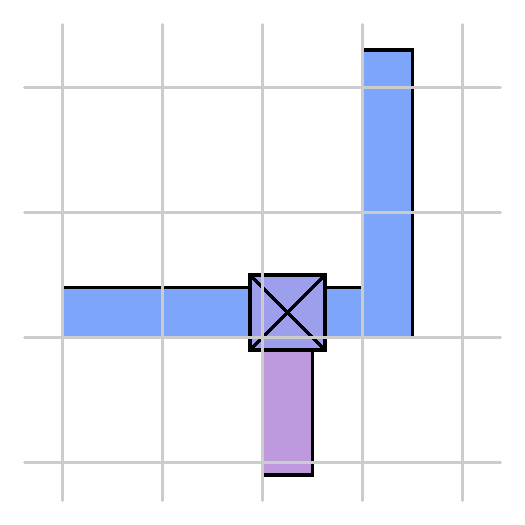
\epsfig{file=../psfigures/tut7.3.ps, width=0.4\columnwidth}
       \caption{When placing hand routing, it is best to place
	wires with their left and bottom edges along grid lines, and
	contacts centered on the wires.  In this fashion, the hand routing
	will block as few routing grid lines as possible.}
   \end{center}
\end{figure}

When placing hand-routing, you can get better routing results
by following the advice illustrated in Figure 3.  First, display
the routing grid.  For example, if the router is using a 8-unit
grid (which is true for the standard SCMOS technology), type
{\bfseries :grid 8}.  Then place all your hand routing with its left
and bottom edges along the grid lines.  Because of the way the
routing tools work, this approach results in the least possible
amount of lost routing space.

\section{More Netlist Commands}

In addition to the netlist menu buttons and commands described
in Section 4, there are a number of other netlist commands you
can invoke by typing in the netlist window.  Many of these
commands are textual equivalents of the menu buttons.  However,
they allow you to deal with terminals by typing the hierarchical
name of the terminal rather than by pointing to it.  If you
don't know where a terminal is, or if you have deleted a label
from your design so that there's nothing to point to, you'll
have to use the textual commands.  Commands that don't just
duplicate menu buttons are described below; see the
{\itshape magic(1)} manual page for details on the others.

The netlist command

\starti
   \ii {\bfseries :extract}
\endi

will generate a net from existing wiring.  It looks under the
box for paint, then traces out all the material in the edit cell
that is connected electrically to that paint.  Wherever the
material touches subcells it looks for terminals in the subcells,
and all the terminals it finds are placed into a new net.  Warning:
there is also an {\bfseries extract} command for layout windows, and it
is totally different from the {\bfseries extract} command in netlist
windows.  Make sure you've got the cursor over the netlist window
when you invoke this command!

The netlist editor provides two commands for ripping up existing
routing (or other material).  They are

\starti
   \ii {\bfseries :ripup} \\
   \ii {\bfseries :ripup netlist}
\endi

The first command starts by finding any paint in the edit cell
that lies underneath the box.  It then works outward from that
paint to find all paint in the edit cell that is electrically
connected to the starting paint.  All of this paint is erased.
({\bfseries :ripup} isn't really necessary, since the same effect can
be achieved by selecting all the paint in the net and deleting
the selection;  it's a hangover from olden days when there was
no selection).
The second form of the command, {\bfseries :ripup netlist}, is similar
to the first except that it starts from each of the terminals
in the current netlist instead of the box.  Any paint in
the edit cell that is electrically connected to a terminal
is erased.  The {\bfseries :ripup netlist} command may be useful to
ripup existing routing before rerouting.

The command

\starti
   \ii {\bfseries :trace} [{\itshape name}]
\endi

provides an additional facility for examining
router feedback.  It highlights all paint connected
to each terminal in the net containing {\itshape name},
much as the {\bfseries Show} menu button does for paint
connected to anything under the box.  The net to be highlighted
may be specified by naming one of its terminals, for example,
{\bfseries :trace shifter/bit[0]/phi1}.
Use the trace command in conjunction with the nets specified in
router feedback to see the partially completed wiring for a net.
Where no net is specified, the {\bfseries :trace} command highlights the
currently selected net.

\end{document}
